\begin{center}
  \Large
  \textbf{WRITER BIOGRAPHY}
\end{center}

\addcontentsline{toc}{chapter}{WRITER BIOGRAPHY}

\vspace{2ex}

\begin{wrapfigure}{L}{0.3\textwidth}
  \centering
  \vspace{-3ex}
  % Ubah file gambar berikut dengan file foto dari mahasiswa
  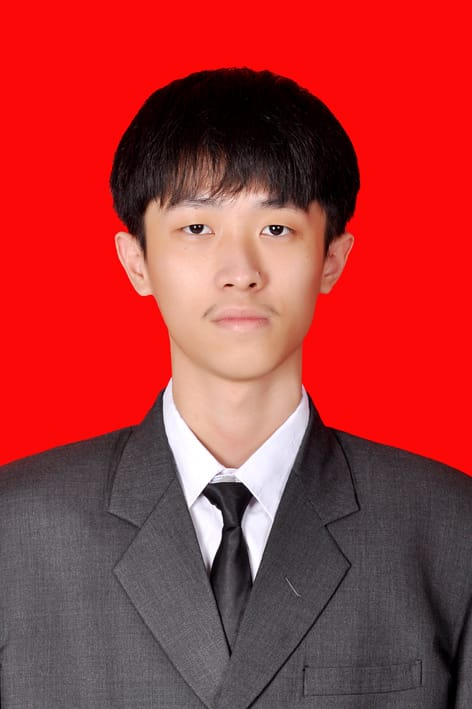
\includegraphics[width=0.3\textwidth]{gambar/nathan.jpg}
  \vspace{-4ex}
\end{wrapfigure}

% Ubah kalimat berikut dengan biografi dari mahasiswa
\name{}, Born in 24 August 2001, a student of Computer Engineering in Sepuluh
Nopember Institute of Technology (ITS) batch 2019. The writer comes from Pasuruan, East Java.
Studied at Sang Timur Catholic Elementery School Pasuruan, Sang Timur Catholic Junior High School Pasuruan,
and St. Louis 1 Senior High School Surabaya. As long as the writer studied in ITS, he was active
in Ichiro Robotics Team as a programmer and B401 Laboratory Assistant. As a part of Ichiro team, the writer has won
some national and international achievements such as National Indonesian Robot Contest 2020 and 2021, FIRA SimulCup 2021 and 2022 that
were held online also National Indonesian Robot Contest 2022 and RoboCup 2022 Bangkok that were held offline.
The writer has joined Bangkit Academy 2022 in Machine Learning Path and had 3 month internship experience in PT Indosat Tbk
in order to complete Bangkit Academy Program. The writer's area of interests in doing the final project are Machine Learning and Computer Vision.
The author can be contacted via email nathanael.hutama24@gmail.com.